%%____________________________________________________________________________||

\section{\texorpdfstring{\znunu\ + jets}{Zinv} background estimation}
\label{sec:zinv}

The irreducible background contribution from the \znunu\ + jets
process can be a sizeable, and often the dominating, contribution in
many event categories of the signal region, particularly at high
\HTmiss. 

%Table~\ref{} (App.~\ref{}) shows % add SM breakdown plots? 
\fixme{Diff w.r.t. old analysis. Heavy flavour.}

\subsection{The ``transfer factor'' method}
\label{sec:tf-method-zinv}

The method used to estimate the \znunuj background relies on the use
of a transfer factor (TF) determined from simulated event samples to
transform the observed event yields in the \mmj sample, categorised
according to \njet and \scalht, $\nobs^{\mmj}(\njet, \scalht)$, into
an estimate of the lost lepton background for the corresponding
(\njet, \scalht) category of the signal region, $\npre^{\znunu}(\njet,
\scalht)$. The categorisation of events according to \njet and \scalht
in the \mmj control region is identical to that for the signal region,
as defined in Sec.~\ref{sec:selection}.\footnote{One detail here is
  that predictions are made according to the \scalht categorisation
  used in the control regions (up to 11 bins), but the predictions are
  then aggregated over a range in \scalht to map onto a coarser
  binning scheme is used in the signal region (up to 5 bins). Further
  details can be found in Sec.~\ref{sec:ht-categorisation}.}  Each
transfer factor is simply a ratio of the yields obtained from Monte
Carlo (MC) simulation for the same (\njet, \scalht) category of the
\mmj control and signal regions:
\begin{equation}
  \label{equ:tf-ratio-zinv}
  {\rm TF} = \frac{N_{\rm MC}^{\znunu}(\njet, \scalht)}{N_{\rm MC}^{\mmj}(\njet, \scalht)} 
\end{equation}

In this way, predictions for the \znunuj background can be made, based
on the \mmj control region, as follows:
\begin{equation}
  \label{equ:pred-method-zinv}
  \npre^{\znunu}(\njet, \scalht) = 
  \frac{N_{\rm MC}^{\znunu}(\njet, \scalht)}{N_{\rm MC}^{\mmj}(\njet, \scalht)} 
  \times 
  \nobs^{\mmj}(\njet, \scalht)   
\end{equation}

The selection criteria for the \mmj control region
(Sec.~\ref{sec:selection}) closely resemble those for the signal
region, differing mainly through the use of a dimuon {\it tag} (that
is ignored in the calculation of jet-based kinematic variables such as
\scalht, \mht, \alphat, \etc) and minimal additional kinematic
requirements (\eg a dimuon invariant mas window) to obtain a sample
enriched in \zmmj events. The same selection criteria are designed to
suppress signal contamination so that unbiased data-driven estimates
for the SM backgrounds in the signal region can be made. Any signal
contamination is accounted for in the likelihood model
(Sec.~\ref{sec:likelihood}).

Figure~\ref{fig:tf_mmZinv} (App.~\ref{app:zinv}) shows the
magnitude of the transfer factors, typically $\ll 1$, The transfer
factors account for differences between the \mmj control and signal
due to the different branching fractions for the decays to neutrinos
or muons, as well as differences in acceptance times efficiency for
the reconstructed muons and extrapolations in kinematic
quantities. For example, the dependence on \njet and \scalht is
largely attributable to the \alphat and \bdphi requirements for the
signal region (that are not used in the \mmj control region).

Many systematic effects are expected to cancel largely in the transfer
factor. However, a systematic uncertainty is assigned to each transfer
factor to account for theoretical uncertainties and effects such as
the mismodelling of kinematics (\eg acceptances) and instrumental
effects (\eg reconstruction efficiencies). These uncertainties are
discussed below. 

\subsection{\texorpdfstring{\nb}{Nb} and \texorpdfstring{\mht}{MHT} templates}

The transfer factors described above provide an estimate of the lost
lepton background as a function of the (\njet, \scalht) category, but
inclusive with respect to \nb and \mht. However, the analysis utilises
the \nb and \mht variables to discriminate effectively between SM
background and \eg a potential contribution from SUSY processes. The
\nb and \HTmiss information is incorporated into the likelihood model
via \nb and \mht templates per (\njet, \scalht) category, $N_{\rm
  MC}^{\ttw}(\nb, \HTmiss;\; \njet, \scalht)$, which is equivalent to
dicing the numerator of the TF according to \nb and \mht, \ie
\begin{equation}
  \label{equ:pred-method-zinv-mht}
  \npre^{\ttw}(\njet, \scalht, \nb, \HTmiss) = 
  \frac{N_{\rm MC}^{\ttw}(\nb, \HTmiss;\; \njet, \scalht)}{N_{\rm MC}^{\mj}(\njet, \scalht)} 
  \times 
  \nobs^{\mj}(\njet, \scalht)
\end{equation}
In this regard, the TFs described in Sec.~\ref{sec:tf-method-zinv}
provide an estimate of the normalisation for each \nb and \mht
template. The \nb and \HTmiss templates are taken from simulation and
the validity of the simulation modelling is tested extensively in the
control regions, as described in Sec.~\ref{sec:mht-zinv}.

\subsection{Sideband normalisation for \texorpdfstring{\zj}{Z+jets}} 
\label{sec:sideband-corrections-zinv}

Corrections to the inclusive cross section used for the \zmmj
simulated samples are determined following a procedure that uses a
binned likelihood fit to data in \HTmiss sidebands of the \mj and \mmj
control regions. Correspondingly, the same corrections are applied to
the \znunuj simulated samples. The procedure is defined in
Sec.~\ref{sec:sideband-corrections}.

As noted previously, this iteration of the analysis is {\em not}
sensitive to whether these corrections are applied or not, due to the
way the transfer factors are constructed. Contrary to the previous
iteration of this analysis, only the \zmmj sample is now used to
predict the \znunuj background.\footnote{In the previous iteration of
  the analysis, all three control regions (\mj, \mmj, and \gj) were
  used to predict the \znunu\ background.} The corrections and
uncertainties for the \zmmj and \znunuj processes, as determined by
the fit, are shown in Table~\ref{tab:sbCorrsFromFit-zinv}.

\begin{table}[!h]
%  \scriptsize
  \centering
  \topcaption{Corrections to the inclusive cross sections 
    for the \zmmj and \znunuj processes determined from a binned
    likelihood fit to data in the $100 < \HTmiss < 200\GeV$ sideband
    to the control regions.}
  \label{tab:sbCorrsFromFit-zinv}
  \begin{tabular}
    {clc}
    \hline
    \textbf{Process} & \textbf{Sample} & \textbf{Corrrection} \\
    \hline
%    \zmmj            & \mmj            & $1.06 \pm 0.01$      \\ % no NLO/NISR
    \zmmj            & \mmj            & $0.91 \pm 0.01$      \\
    \znunuj          & (\mmj as proxy) & $0.91 \pm 0.01$      \\
    \hline
  \end{tabular}
\end{table}


\subsection{Overview of systematic uncertainties}
\label{sec:systematics-zinv}

The following sections address the estimation of systematic
uncertainties related to the \znunuj background estimation. All
relevant uncertainties are listed in Table~\ref{tab:systs-zinv}, along
with their representative magnitudes and assumptions on inter-bin
correlations. How the uncertainties are incorporated into the
likelihood model is described in Sec.~\ref{sec:likelihood}.

\begin{table}[h!]
  \caption{Sources of systematic uncertainty in the transfer factors
    used to estimate the \znunuj background using the \mmj control
    region. Also shown are the nuisance parameters and correlation
    scheme, as well as representative magnitudes for the uncertainties
    [\%]. The ``type'' refers to whether the nuisance parameters are
    unique to the \znunuj background or shared with the lost lepton 
    background estimate (see Table~\ref{tab:systs-ttw}). 
  }   
  \label{tab:systs-zinv}
  \centering
  \fontsize{8}{9.6}\selectfont
  \begin{tabular}{ llllc }
    \hline
    Source of uncertainty               & Nuisance parameters / correlation              & Magnitude (\%)               & Shared & Figure                              \\
    \hline
    Finite-size simulated samples       & 1 per (\njet, \scalht, \nb, \mht) category     & 1--100                       & Unique & n/a                                 \\
    Minimum bias cross section (pileup) & 1, correlated across \njet, \scalht, \nb, \mht & 2.3--2.8                     & Shared & \ref{fig:tfSyst_pu_mmZinv}          \\
    $\mu_R$ / $\mu_F$ scales            & 1, correlated across \njet, \scalht, \nb, \mht & X--Y                         & Shared & \ref{fig:tfSyst_scale_mmZinv}       \\
    Parton density functions            & 1, correlated across \njet, \scalht, \nb, \mht & X--Y                         & Shared & \ref{fig:tfSyst_pdf_mmZinv}         \\
    QCD + EWK NLO corrections           & 1, correlated across \njet, \scalht, \nb, \mht & 2.2--14.3                    & Shared & \ref{fig:tfSyst_nlo_mmZinv}         \\
    Signal trigger efficiency           & 1, correlated across \njet, \scalht, \nb, \mht & 0.0--2.0                     & Shared & \ref{fig:tfSyst_trigger_mmZinv}     \\
    Lepton efficiency (selection)       & 1, correlated across \njet, \scalht, \nb, \mht & 0.0--4.2                     & Unique & \ref{fig:tfSyst_muonsf_mmZinv}      \\
    Lepton efficiency (veto)            & 1, correlated across \njet, \scalht, \nb, \mht & X--Y                         & Unique & \ref{fig:tfSyst_leptonveto_mmZinv}  \\
    Jet energy scale                    & 1, correlated across \njet, \scalht, \nb, \mht & 5.3--8.0                     & Shared & \ref{fig:tfSyst_jec_mmZinv}         \\
    b-quark tag efficiency              & 1, correlated across \njet, \scalht, \nb, \mht & 0.3--0.6                     & Shared & \ref{fig:tfSyst_bsf_mmZinv}         \\
    b-quark mistag probability          & 1, correlated across \njet, \scalht, \nb, \mht & 0.2--1.8                     & Shared & \ref{fig:tfSyst_bsfl_mmZinv}        \\
    \alphat + \bdphi extrapolation      & 1 per \njet category, 1 per \scalht category   & X--Y (\njet), X--Y (\scalht) & Unique & \ref{fig:closure_AlphaT_bDPhi_mumu} \\
%    \alphat extrapolation              & 1 per \njet category, 1 per \scalht category   & X--Y (\njet), X--Y (\scalht) & Unique & \ref{fig:closure_AlphaT_mumu}       \\
%    \bdphi extrapolation               & 1 per \njet category, 1 per \scalht category   & X--Y (\njet), X--Y (\scalht) & Unique & \ref{fig:closure_bDPhi_mumu}        \\
    \hline
  \end{tabular}
\end{table}

Several sources of uncertainty are evaluated.  The most relevant
effects are discussed below, and generally fall into one of two
categories. The first category concerns known theoretical and
experimental effects that are propagated through to the transfer
factors and \HTmiss templates. These are decribed in
Sec.~\ref{sec:mc-variations-zinv}. The second set can be considered as
``known unknowns'' that are derived from dedicated ``closure test''
and \HTmiss-modelling studies that involve confronting transfer
factors determined in the phase space of this search against data in
the control regions. This latter category of uncertainties are
summarised in Secs.~\ref{sec:closure-tests-zinv} and
\ref{sec:mht-zinv}.

\subsection{Known theoretical and experimental uncertainties}
\label{sec:mc-variations-zinv}

Most of the uncertainties considered for the determination of the lost
lepton background, described in Sec.~\ref{sec:mc-variations} are also
considered here. The same treatment and assumptions are made. Below,
we simply highlight relevant behvaviours and reference the
corresponding figures. 

\subsubsection{Minimum bias cross section / pileup}
\label{sec:tfSyst_pu-zinv}

The relative change in the transfer factors under this variation is
small, at the few percent level, as shown in
Fig.~\ref{fig:tfSyst_pu_mmZinv} (App~\ref{app:zinv}).

\subsubsection{Effect of scale and PDF on lepton acceptance}
\label{sec:tfSyst_pdf-zinv}

Figures~\ref{fig:tfSyst_scale_mmZinv} and \ref{fig:tfSyst_pdf_mmZinv}
(App.~\ref{app:zinv}) show the behaviour in the transfer factors for
variations in scale and PDF, respectively.

\subsubsection{Missing higher-order corrections in LO \texorpdfstring{\MADGRAPH}{MadGraph}
  samples}
\label{sec:nlo-zinv}

The \zmmj and \znunuj processes are generated at leading order with
the \MADGRAPH code. The effect of missing higher-order QCD and EWK
corrections are studied by considering the effect of
LO$\rightarrow$NLO corrections, determined as a function of Z boson
\Pt and shown in in Fig.~\ref{fig:tfSyst_nlo_mmZinv}
(App.~\ref{app:zinv}), on the transfer factors and \HTmiss templates.

Simulated \zmmj and \znunuj events are weighted according to these NLO
corrections, and the magnitude of each correction is propagated as an
uncertainty throughout the analysis. Fig.~\ref{fig:tfSyst_nlo_mmZinv}
(App.~\ref{app:zinv}) show the effect on the transfer factors as a
function of the various discriminating variables. Uncertainties are
typically at the percent level and as large as $\sim 15\%$.

\subsubsection{Signal trigger uncertainty}
\label{sec:tfSyst_trigger-zinv}

The relative change in the transfer factors is typically at the few
percent level, as presented in Fig.~\ref{fig:tfSyst_trigger_mmZinv}
(App~\ref{app:zinv}).

\subsubsection{Lepton trigger / identification / isolation efficiencies}
\label{sec:leptonSyst-zinv}

Figures~\ref{fig:tfSyst_muonsf_mmZinv} and
\ref{fig:tfSyst_leptonveto_mmZinv} (App.~\ref{app:zinv}) show the
systematic uncertainties associated with the data/simulation scale
factors related to the trigger, identification, and isolation
efficiencies for muon selection and identification and isolation
efficiencies for lepton veto, repectively.

\subsubsection{Jet energy scale}
\label{sec:tfSyst_jec-zinv}

The relative change in the transfer factors is presented as a function
of \scalht and jet category in Fig.~\ref{fig:tfSyst_jec_mmZinv}
(App.~\ref{app:zinv}). The changes are typically in the range of
$5-8\%$.

\subsubsection{B-tagging efficiency and mistag probability}
\label{sec:tfSyst_btag-zinv}

The relative change in the transfer factors is presented as a function
of \scalht and jet category in Figs.~\ref{fig:tfSyst_bsf_mmZinv} and
\ref{fig:tfSyst_bsfl_mmZinv} (App.~\ref{app:zinv}).  They are
typically in the range of $0-2\%$.

\subsection{Systematics uncertainties in transfer factors from closure tests}
\label{sec:closure-tests-zinv}

As described in Sec.~\ref{sec:closure-tests}, a second category of
uncertainty is determined from sets of closure tests based on data
control samples~\cite{RA1Paper2012}. The tests relevant to the \znunuj
background estimate are listed below. 

\subsubsection{Extrapolation in \texorpdfstring{\alphat}{AlphaT} and
  \texorpdfstring{\bdphi}{biased dPhi}}
\label{sec:tfSyst_alphaT-zinv}

Events in the \mmj control region are not required to satisfy any
requirement on \alphat or \bdphi. Hence, the accuracy of the modelling
of the the \alphat and \bdphi variables are estimated using the \mmj
sample using dedicated closure tests that confront data yields in a
subsample of \mmj events, satisfying the \alphat and/or \bdphi
requirements, against predictions that are determined using another
subsample of \mmj events that satisfy an inverted requirement on
\alphat and/or \bdphi. Further details of the procedure are found in
Sec.~\ref{sec:closure-tests}. 

The level of closure for an extrapolation in \alphat (only) with the
\mj sample is shown in Fig.~\ref{fig:closure_AlphaT_mu}
(App.~\ref{app:zinv}) as function of \scalht and \njet. Similarly,
Fig.~\ref{fig:closure_bDPhi_mu} (App.~\ref{app:zinv}) shows the same
information for the extrapolation in \bdphi (only). Finally, the level
of closure observed when both \alphat and \bdphi requirements are
simultaneously imposed is summarised in
Fig.~\ref{fig:closure_AlphaT_bDPhi_mu} (App.~\ref{app:zinv}).

Any non-closure in the extrapolation of both \alphat and \bdphi is
covered by a systematic uncertainty, which is defined as the
quadrature sum of the observed non-closure and its statistical
uncertainty (indicated by the blue histogram in the figures). 

\subsection{Systematics uncertainties in the \texorpdfstring{\HTmiss}{MHT} templates}
\label{sec:mht-zinv}

The modelling of the \mht variable for the \znunuj background is
performed with the \mmj sample as a proxy. Discussion and motivation
for these tests of the \mht modelling against data are provided in
Sec.~\ref{sec:mht}. Here, for brevity, only the figures are
summarised.

The figures in App.~\ref{app:mht-zinv} show the ratio of events
obtained from data and simulation as a function of \mht based on a
sample of \mj events that are {\it categorised} according to \njet,
\scalht, and \nb. Note that the \scalht categorisation scheme of the
control regions (Sec.~\ref{sec:ht-categorisation}) is used in this
validation of the \mht modelling. The \nb categorisation is not
relevant for this discussion.

\begin{figure}[h!]
  \centering
  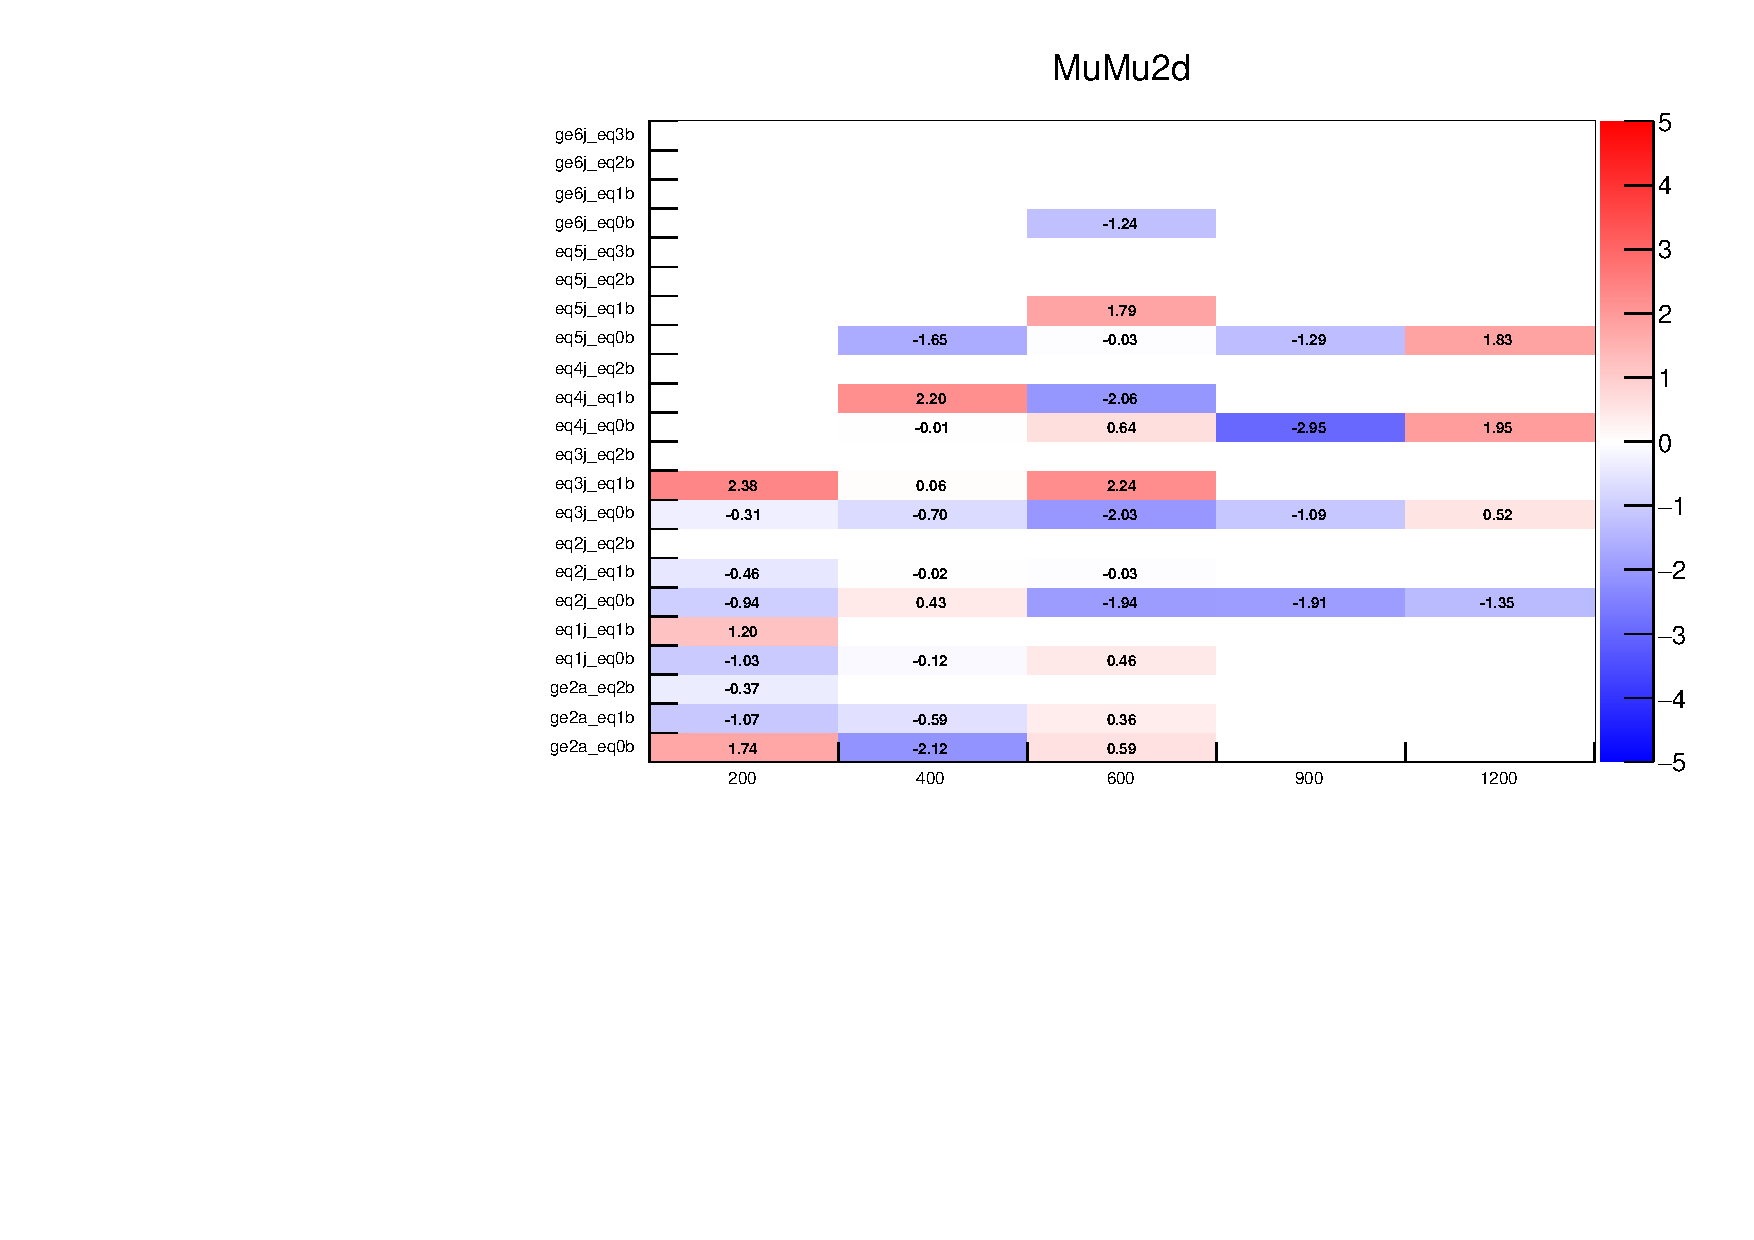
\includegraphics[width=0.5\textwidth]{figures/mhtTemplate/exclusive/MuMu_2D}~
  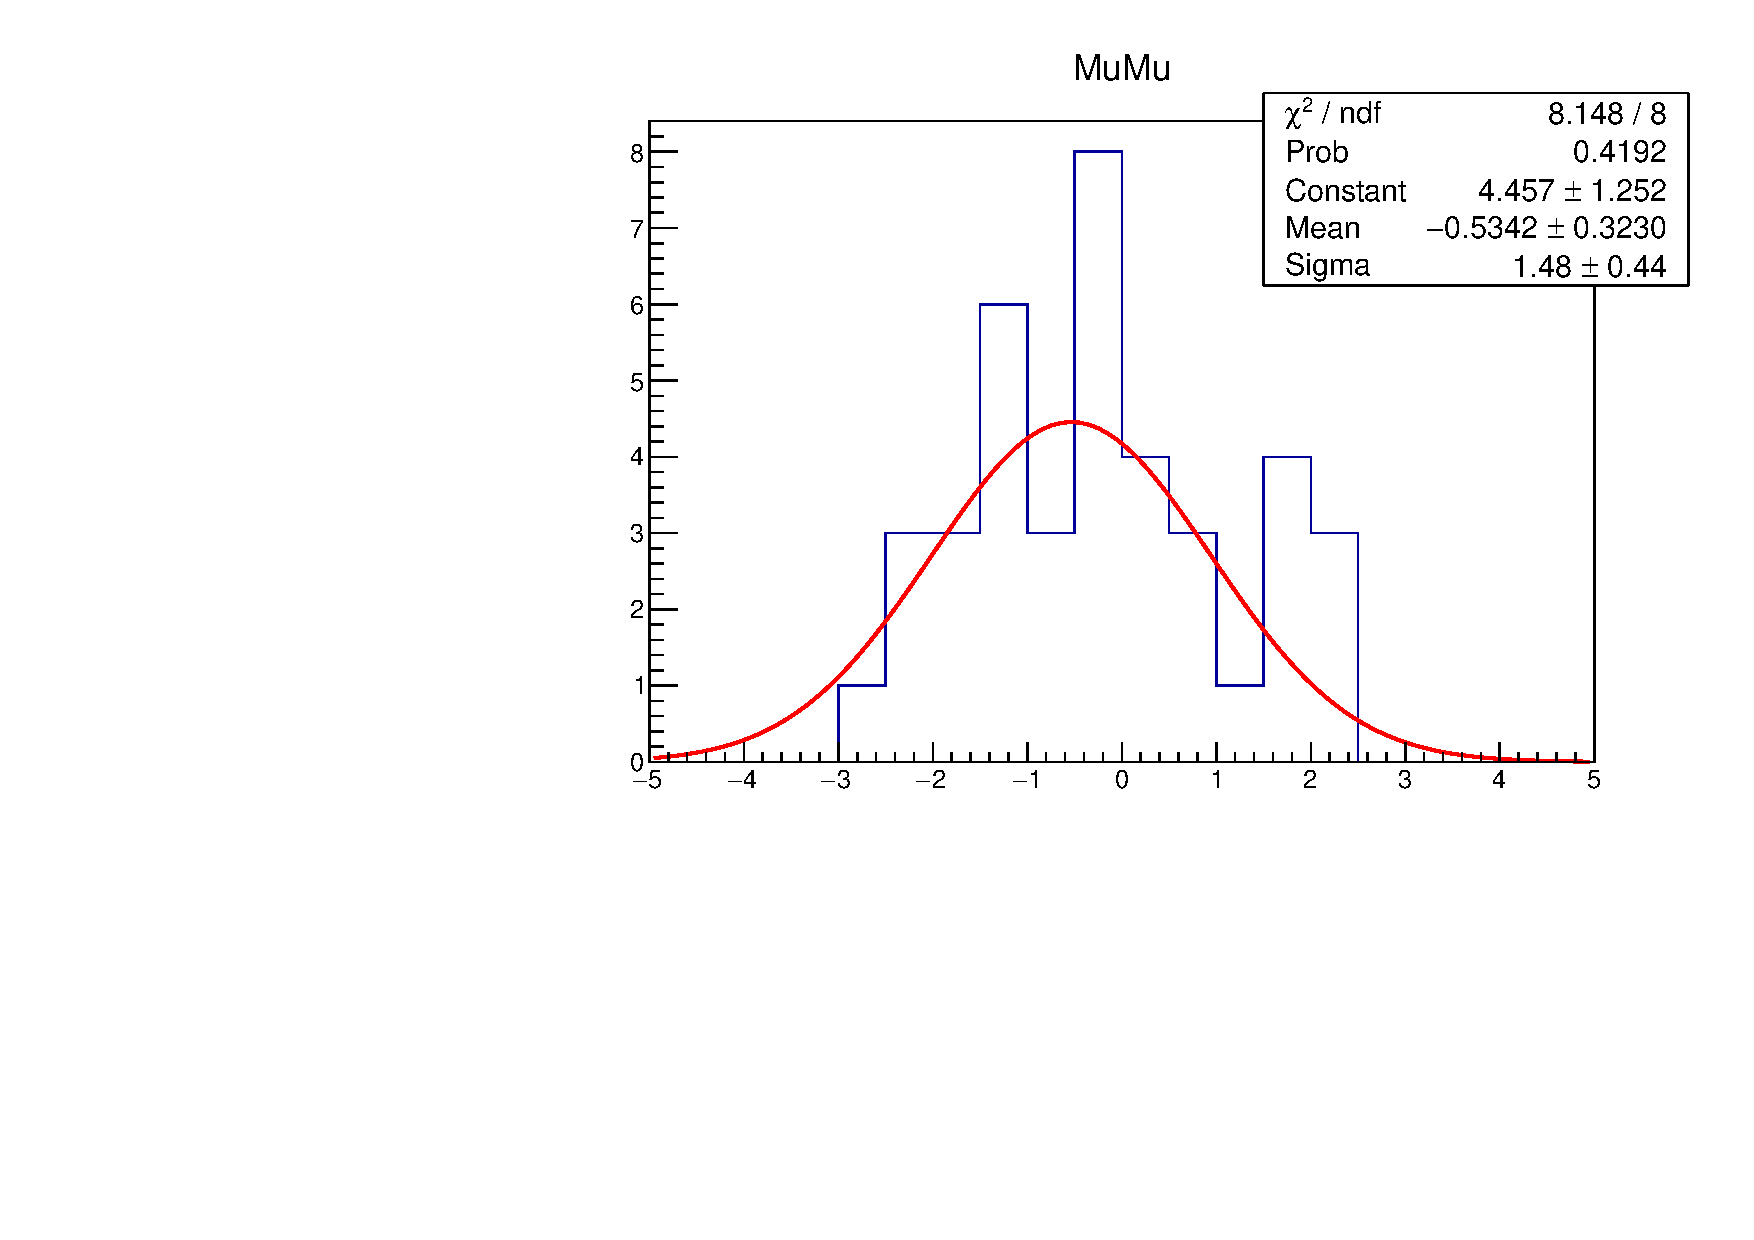
\includegraphics[width=0.5\textwidth]{figures/mhtTemplate/exclusive/MuMu}\\
  \caption{(Left) The best fit value for the linear parameter
    relative to unity in units of the associated statistical
    uncertainty, \ie the statistical ``pull'', as a function of \njet,
    \nb, and \scalht. (Right) The histogram of the pull values.}
  \label{fig:pulls-zinv} 
\end{figure}

The fit information in the figures of App.~\ref{app:mht-zinv} is
summarised in Fig.\ref{fig:pulls} (left), which shows the best fit
value for the linear parameter (of the first-order orthogonal
polynomial) relative to unity (\ie no trend) in units of the
associated statistical uncertainty, \ie the statistical ``pull'', as a
function of \njet, \nb, and \scalht. As for the studies based on the
\mj sample, the pulls appear not to exhibit any structure as a
function of \njet, \nb, nor \scalht, and are approximately
gaussian-distributed, with a mean and width compatible with zero and
unity, respectively. This indicates that no large, significant bias is
found in the simulation modelling of the \mht variable when events are
categorised by \njet, \scalht, and \nb. (The same conclusion is also
reached without categorising by \nb.)
\begin{figure}[h!]
  \centering
  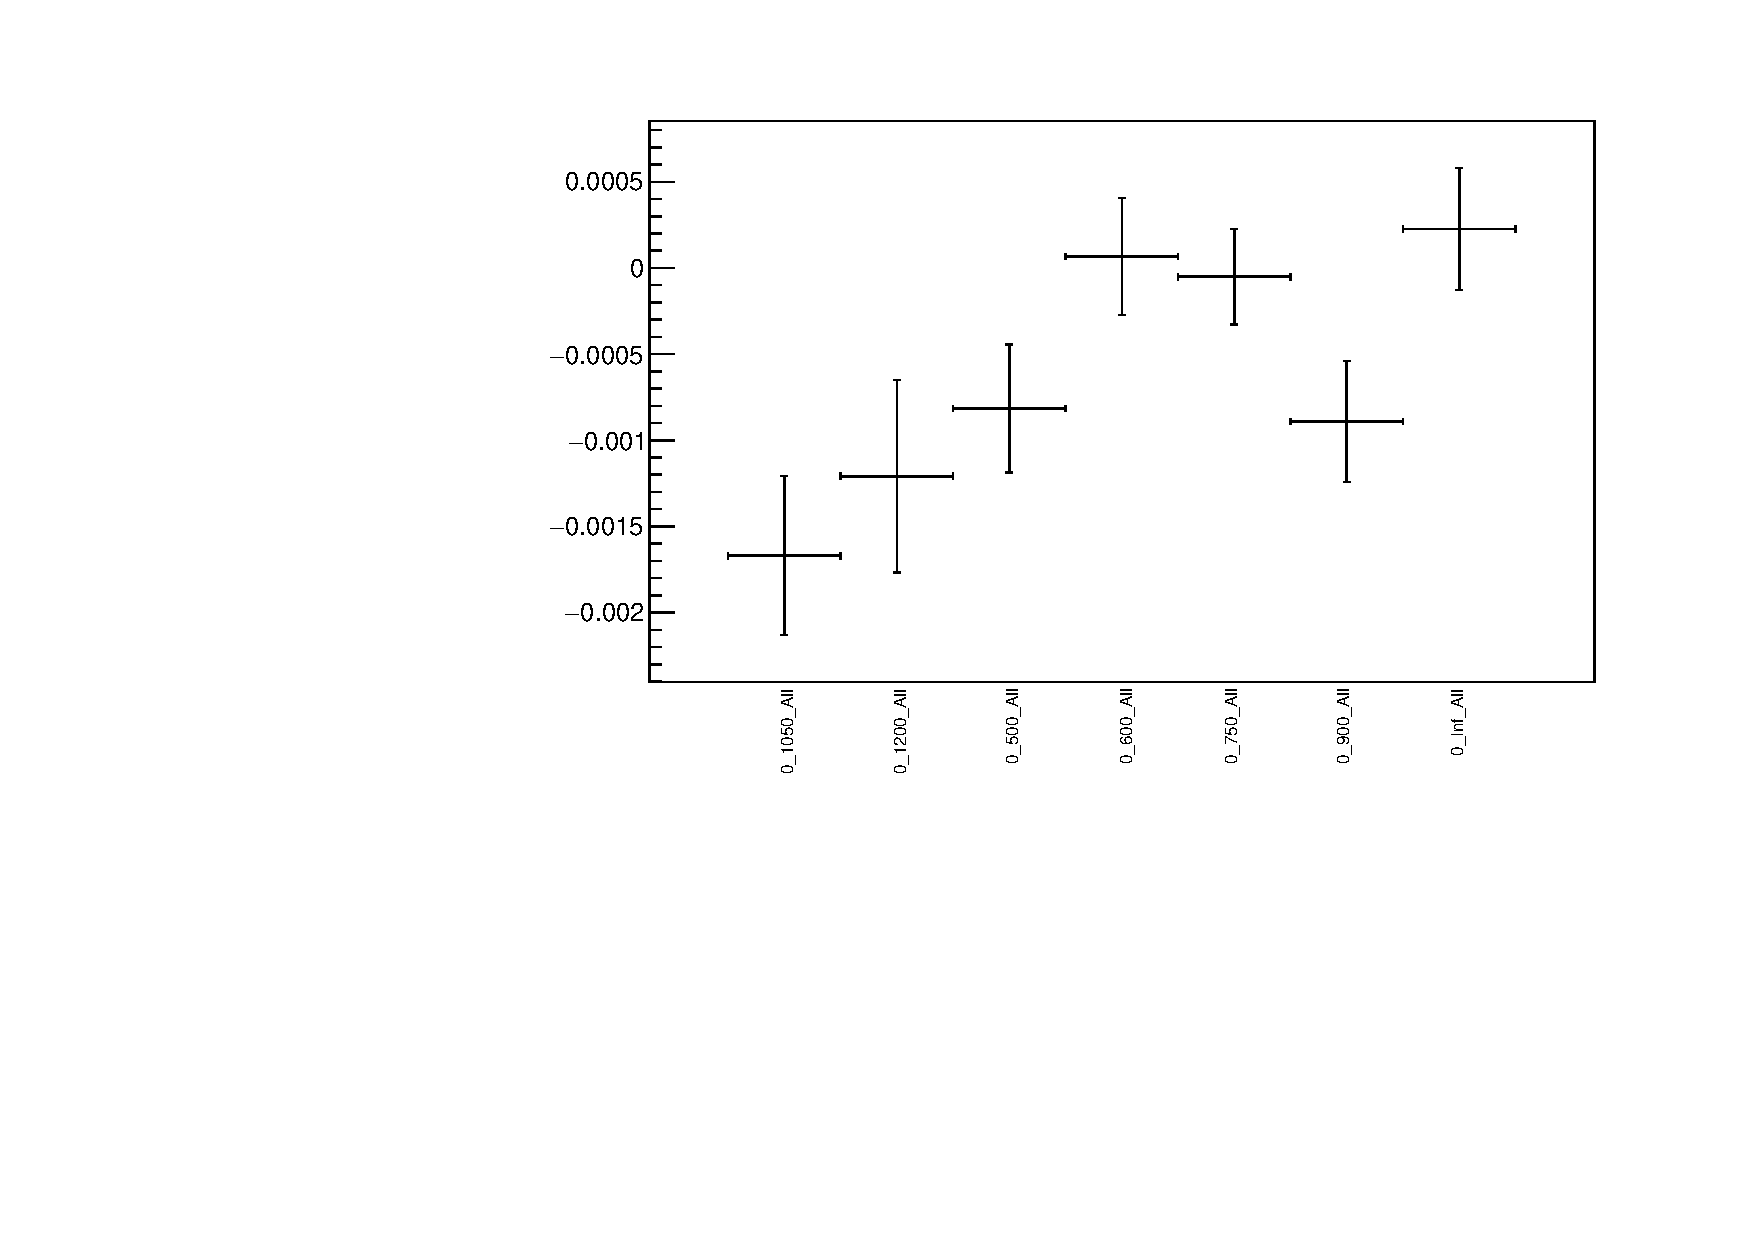
\includegraphics[width=0.5\textwidth]{figures/mhtTemplate/exclusive_corr_njet/MuMu_graph}~
  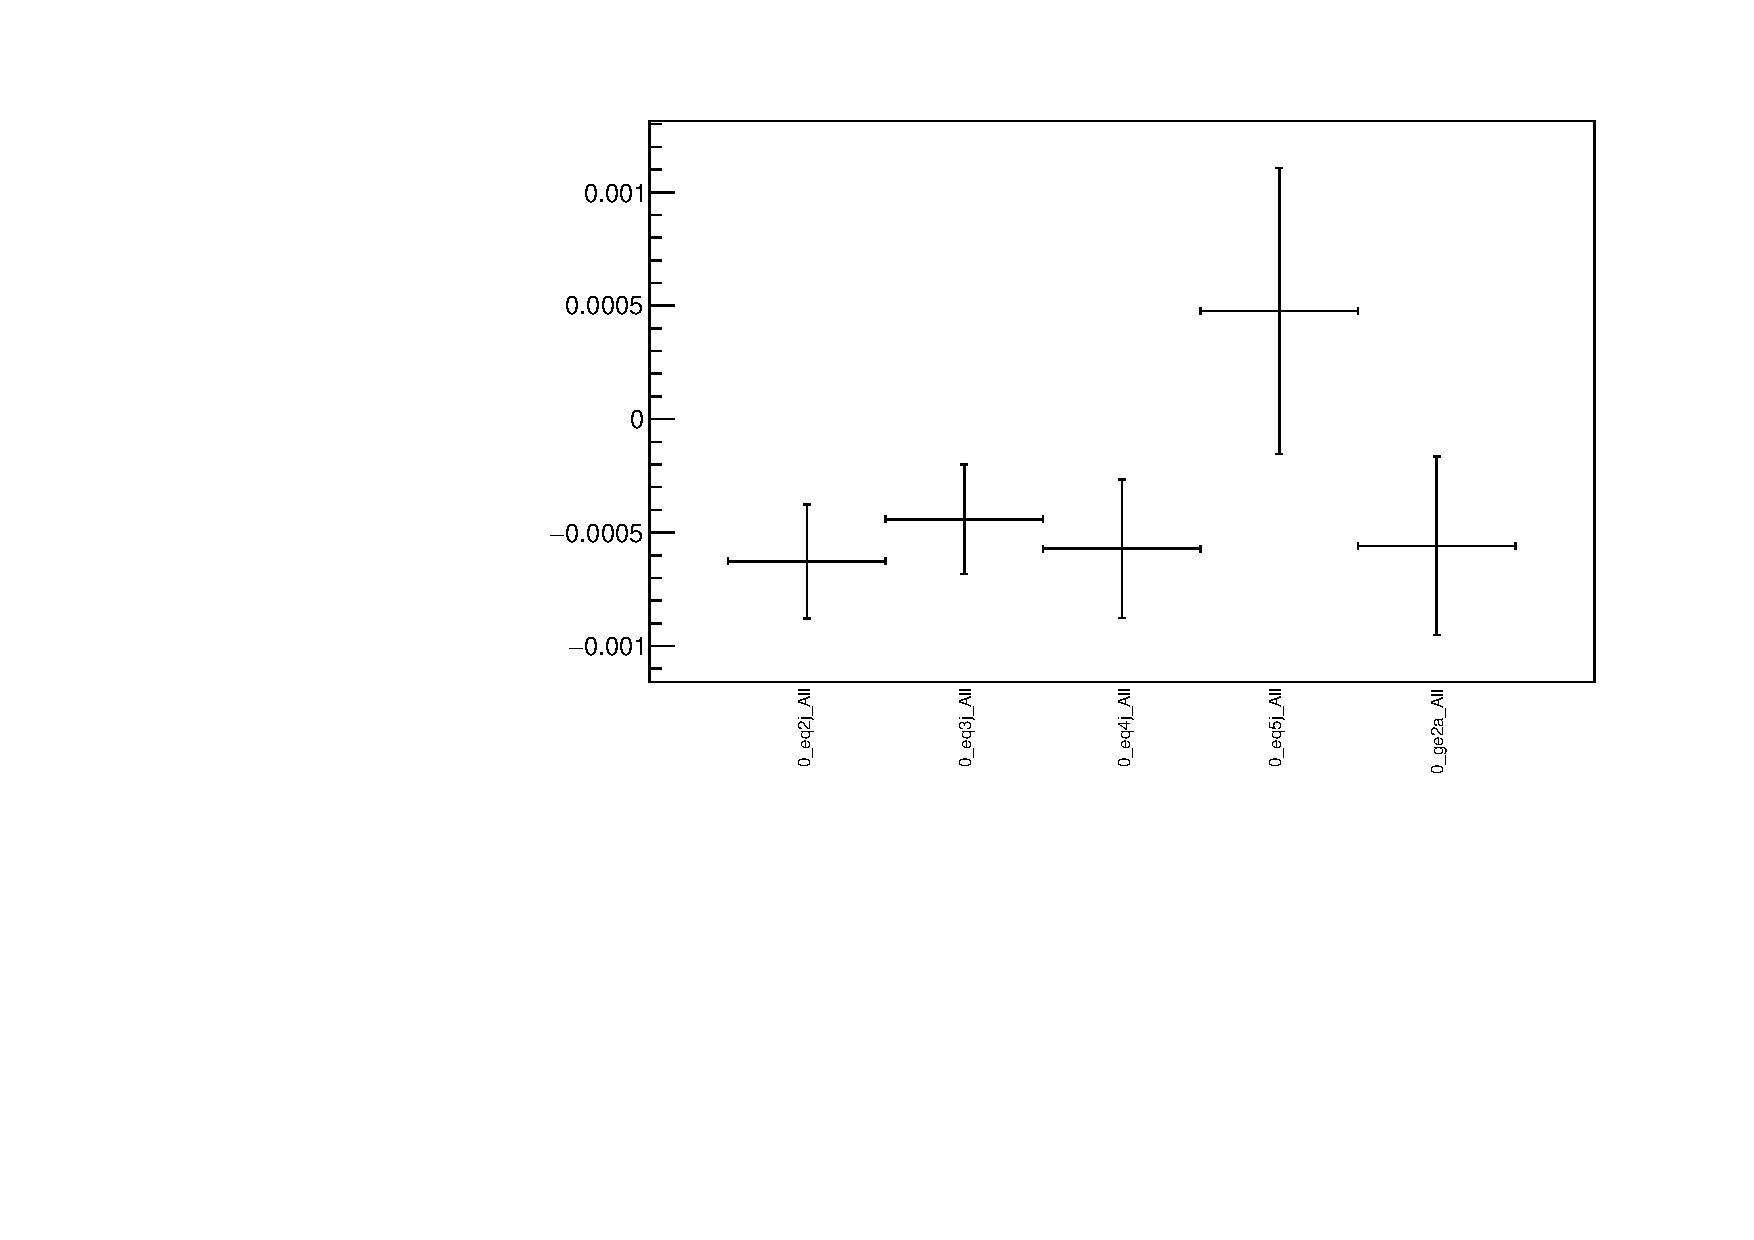
\includegraphics[width=0.5\textwidth]{figures/mhtTemplate/exclusive_corr_ht/MuMu_graph}\\
  \caption{\label{fig:postFitMuMu} Post fit values and uncertainties of
    the linear parameters used to determine the systematics,
    correlated in (left) \njet and (right) \scalht.}
\end{figure}

\begin{figure}[h!]
  \centering
  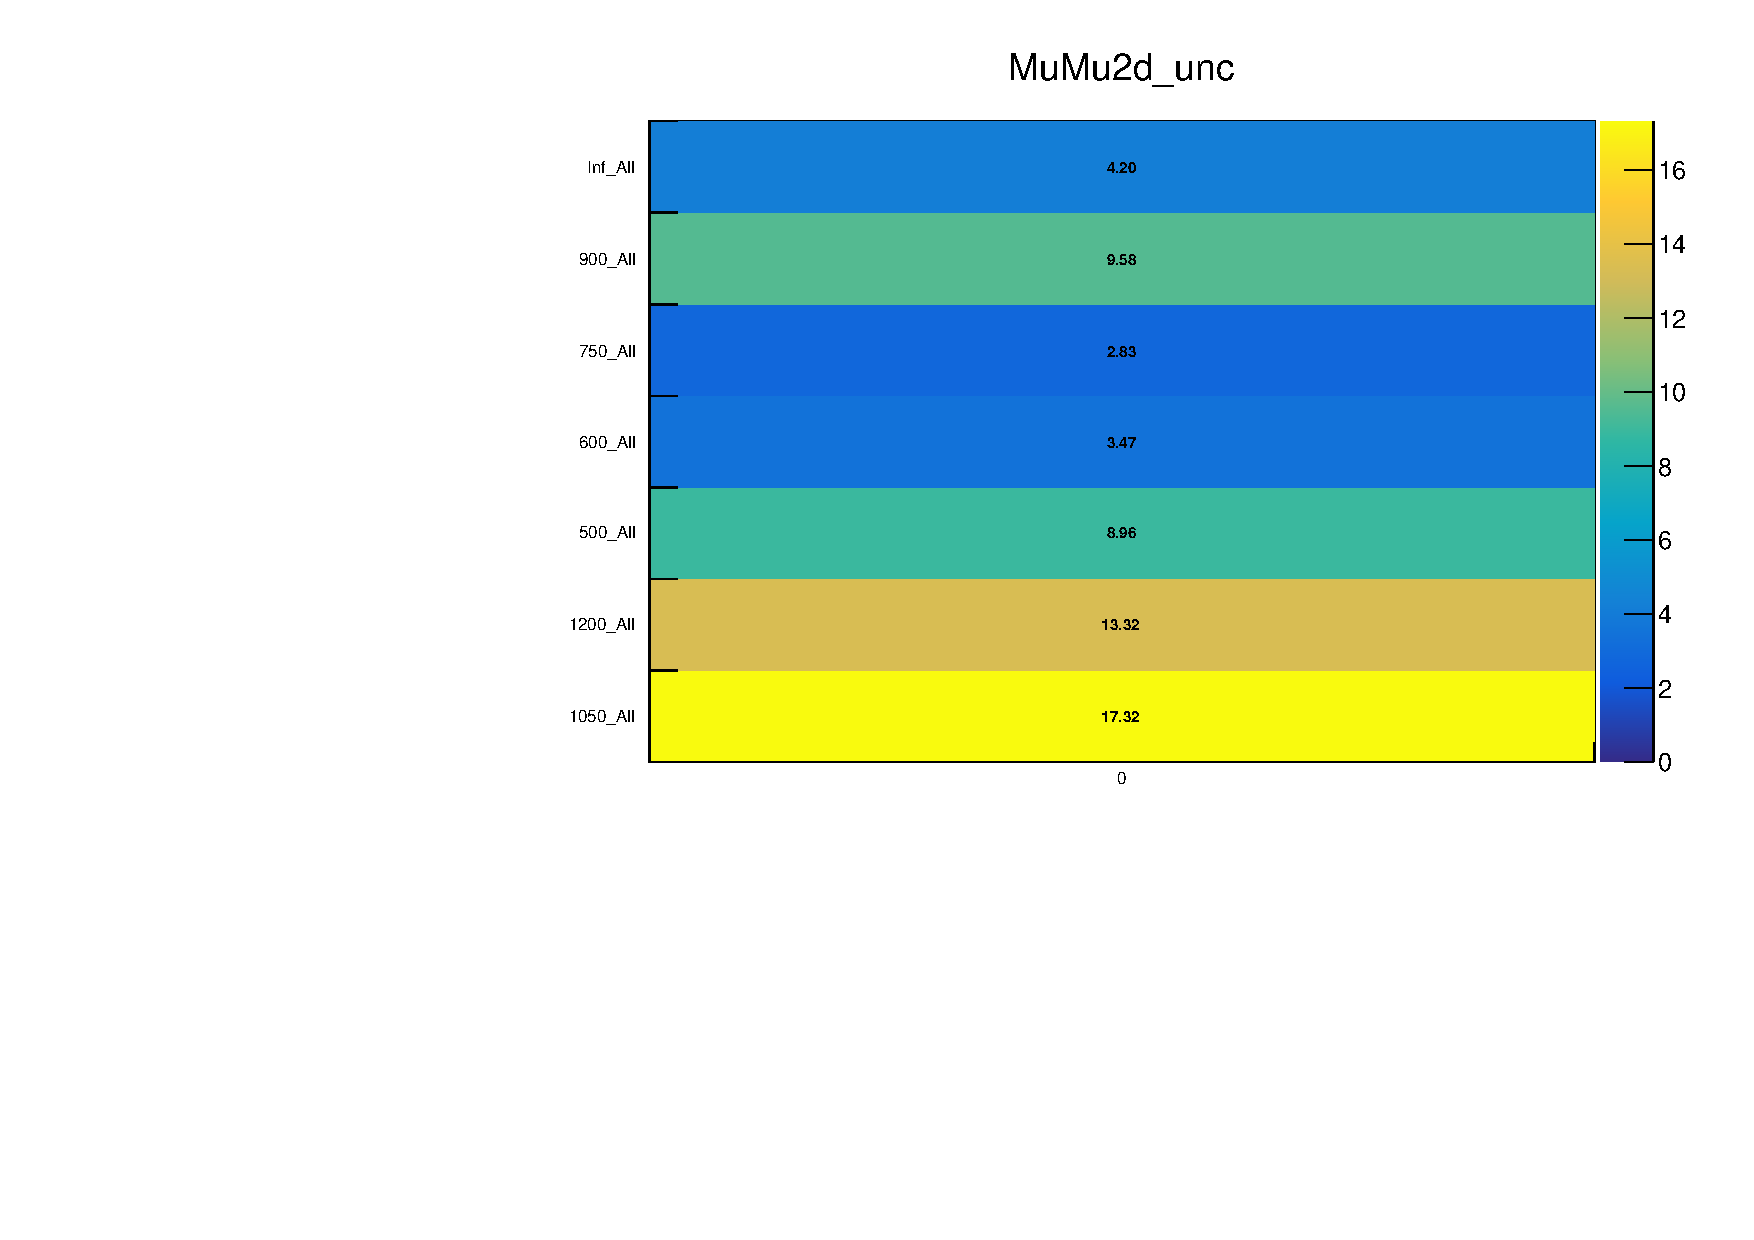
\includegraphics[width=0.5\textwidth]{figures/mhtTemplate/exclusive_corr_njet/MuMu_2D_unc}~
  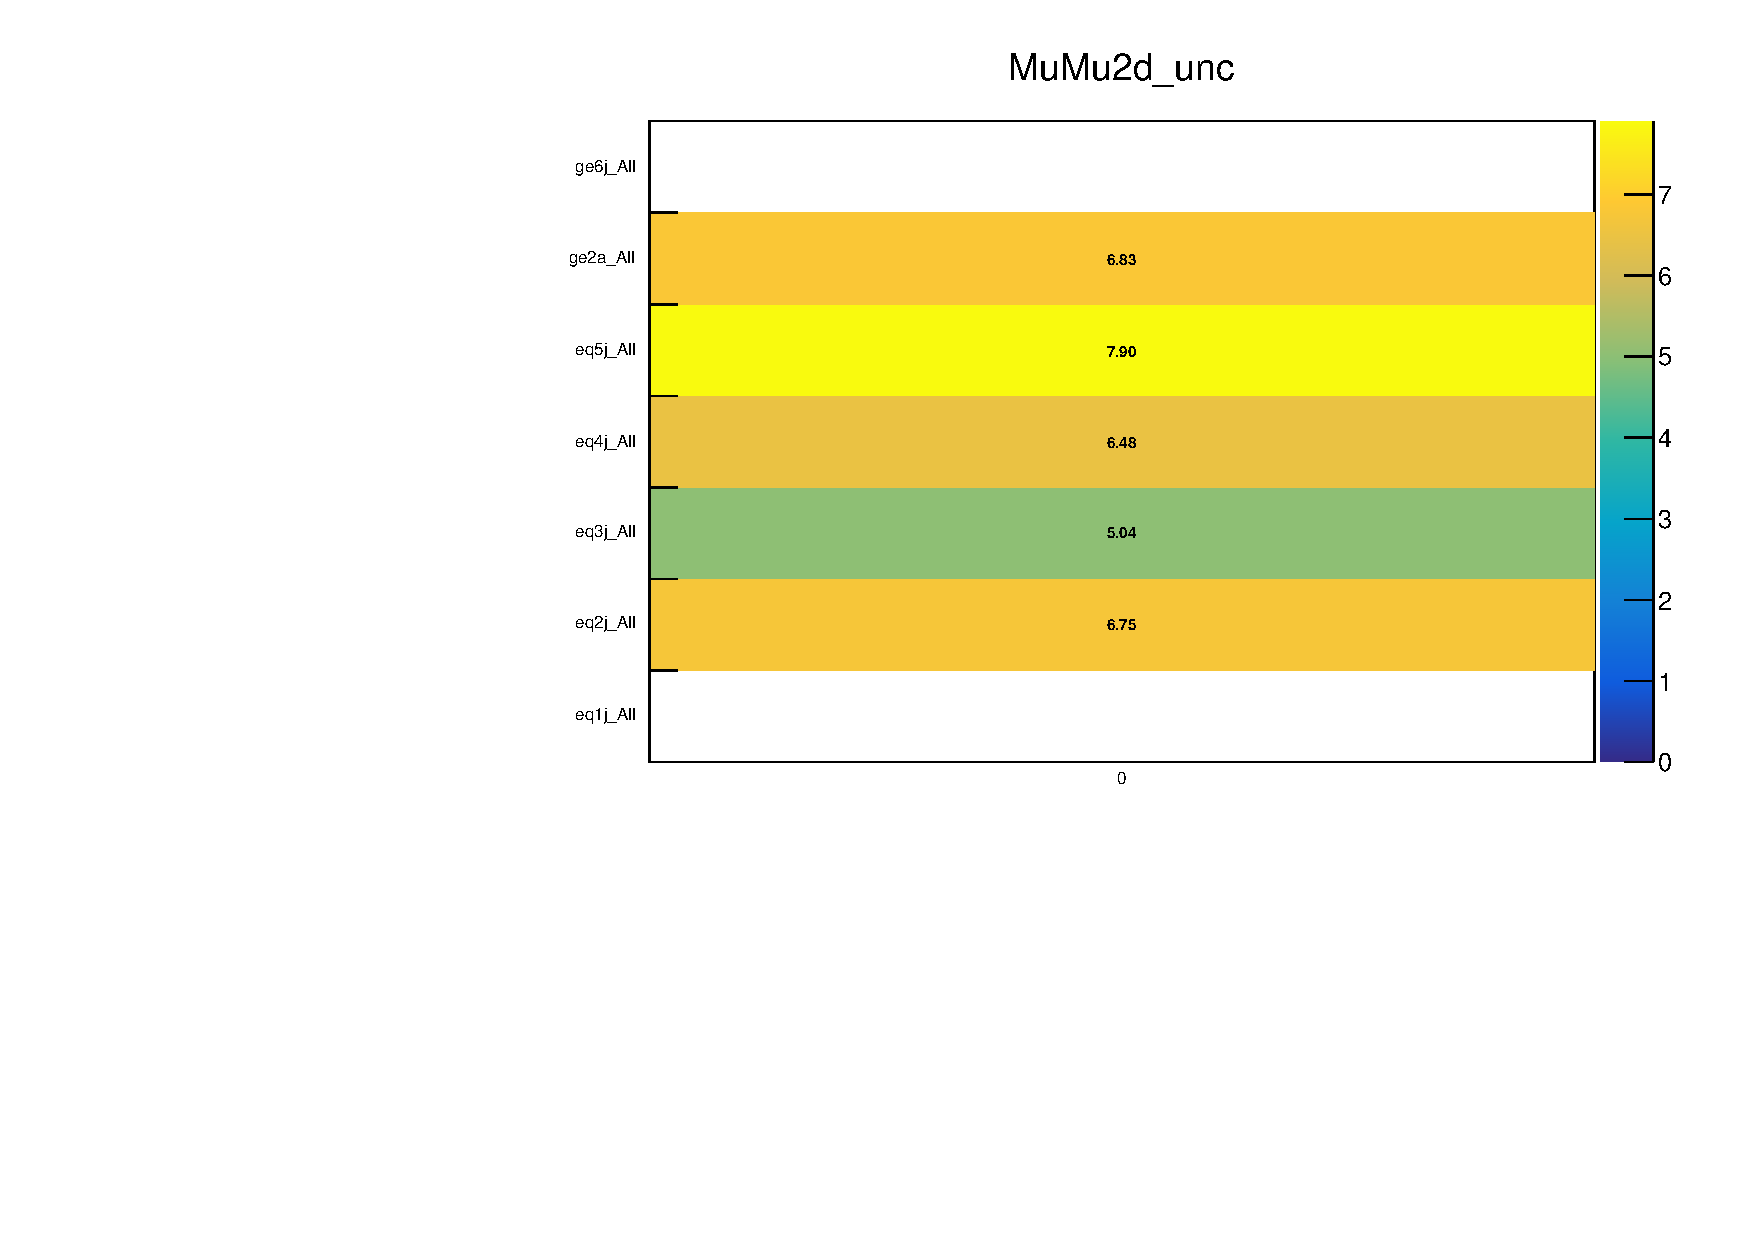
\includegraphics[width=0.5\textwidth]{figures/mhtTemplate/exclusive_corr_ht/MuMu_2D_unc}\\
  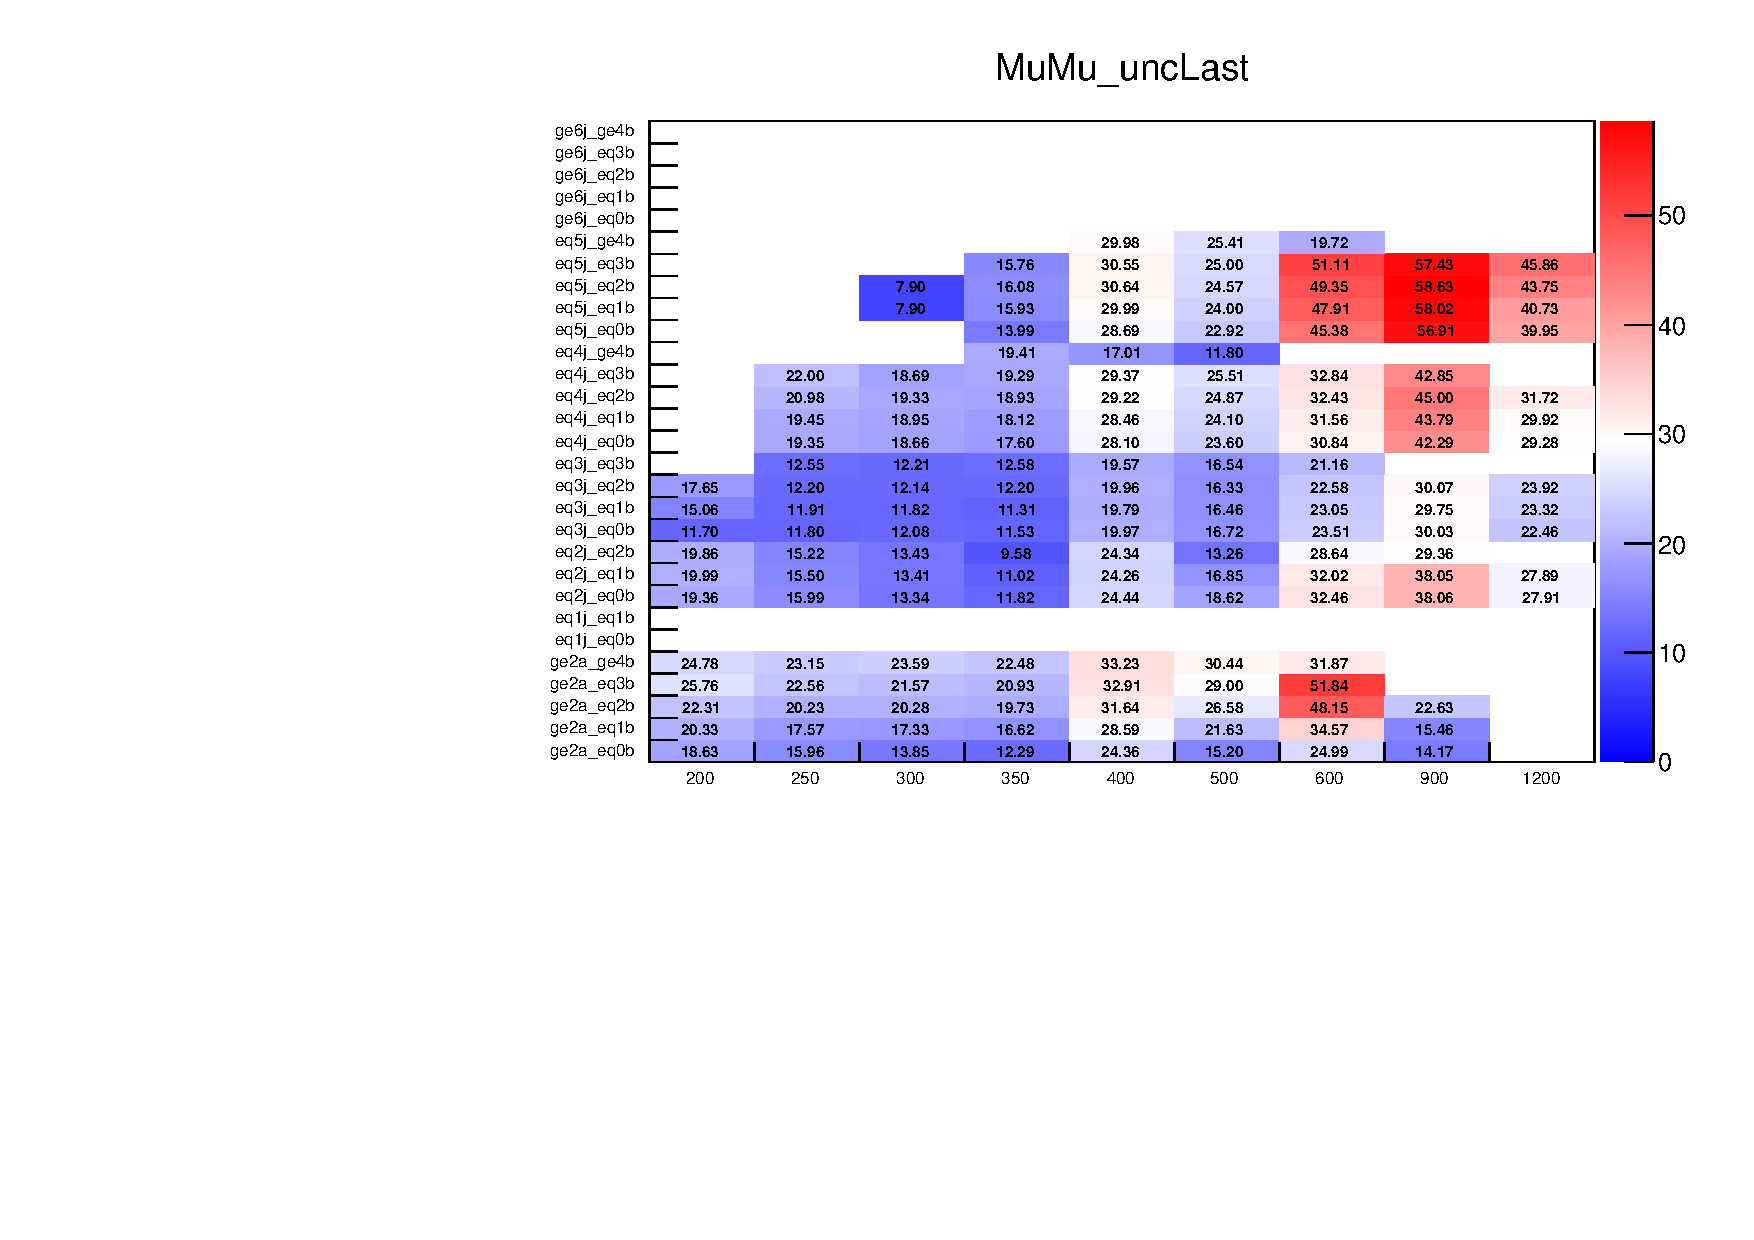
\includegraphics[width=0.5\textwidth]{figures/mhtTemplate/exclusive_corr_ht/MuMu_uncLast}\\
  \caption{\label{fig:postFitErrMuMu} Systematic uncertainties (\%) per
    100\GeV-interval in \mht for effects correlated in (left) \njet
    and (right) \scalht, as determined in the \mj control
    region. (Bottom) Also shown is the systematic uncertainty (\%) in
    the final open \mht bin for each (\njet, \scalht, \nb) category.}
\end{figure}

The procedure described in Sec.~\ref{sec:mht_syst_mu} is used to
determine the systematic uncertainties in the \mht
modelling. Figure~\ref{fig:postFitMuMu} summarises the post-fit values
and uncertainties of the linear parameters of the orthogonal
polynomials. Figure~\ref{fig:postFitErrMuMu} shows the systematic
uncertainty assumed per 100\GeV-interval in \mht due to effects
correlated in (left) \njet and (right) \scalht, as determined in the
\mj control region. The values are at the few percent level. Finally,
Figure~\ref{fig:postFitErrMuMu} also shows the systematic uncertainty
in the final open \mht bin for each (\njet, \scalht, \nb) category,
which is typically at the level of 5--20\%.
